\newpage
\subsection{Fatigue verification of a winch}
	
	\paragraph{Problem} A winch is used for the storage of small boats; the driving torque is applied to the shaft by means of a chain transmission. The winch drum is fitted  onto the shaft (refer to figure \ref{ex:boat}).\\
	It is requested to devise a model of analysis for the identification of the stress state in the shaft and the nominal stress state at critical points. On the basis of the analysis verification, the shaft must be verified for fatigue assuming with reasonable approximation the most critical configuration for the length $L_x$.
	
	Geometrical dimensions known: $D_c = 250mm, D_d = 150mm, D_1 = 50mm, D_2 = 60mm, D_3 = 50mm, L_1 = 200mm, L_2 = 240mm, L_3 = 320mm, L_4 =16mm, L_5 = 250mm, s = 20mm, \alpha = 25^\circ$; the radii of the shoulders are $r=2mm$. Boats are considered to have mass $m=600kg$ and the friction coefficient between boat and terrain $f_{bt} = 0.15$. The shaft has a ground surface finish and has the following material property: $\suts= 700MPa, \sys = 450 MPa,\sigma_{lim} = 360MPa$ (fully reversed bending).
	
	\begin{figure}[bh]
		\centering 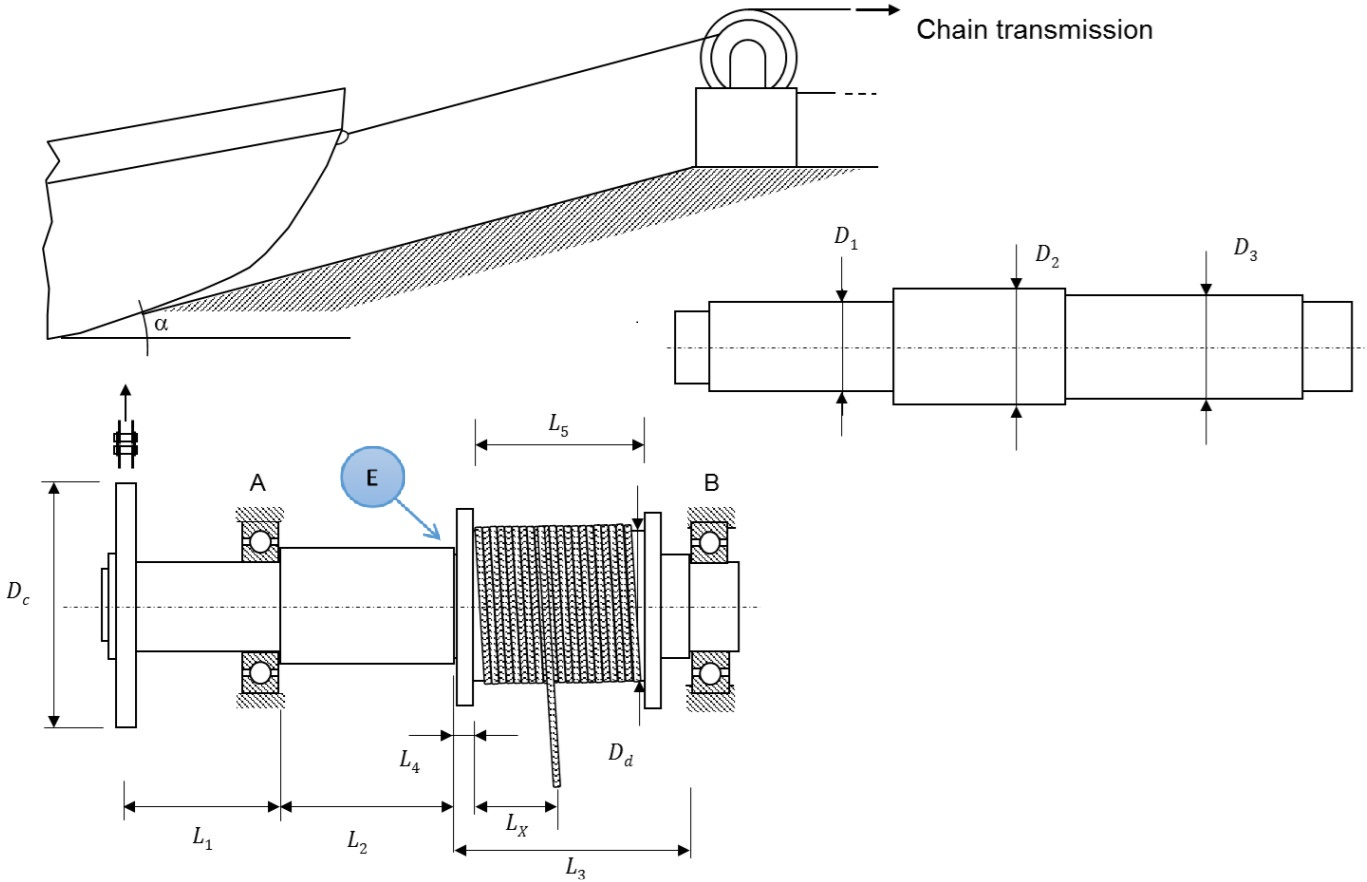
\includegraphics[width=0.9\linewidth]{boat-ex}
		\caption{sketch of the winch lifting a boat.} \label{ex:boat}
	\end{figure}

	\paragraph{Solution} The first thing to do is determine the action exchanged between the boat and the winch; considering figure \ref{ex:boat-a} the force $F_r$ acting on the drum must equation action along the $x'$ axis in figure, and so
	\[ F_r = mg \sin \alpha + f_{bt} mg \cos \alpha = 3\,287.71 N\]
	Equating the torque transmitted on the shaft allows to explicit the force $F_c$ applied by the chain:
	\[ F_c r_c = F_r r_d \qquad \Rightarrow \quad F_c = F_r \frac{r_d}{r_c} = F_r \frac{D_d}{D_c} = 1\,972.63 N\]
	\begin{figure}[bt]
		\centering 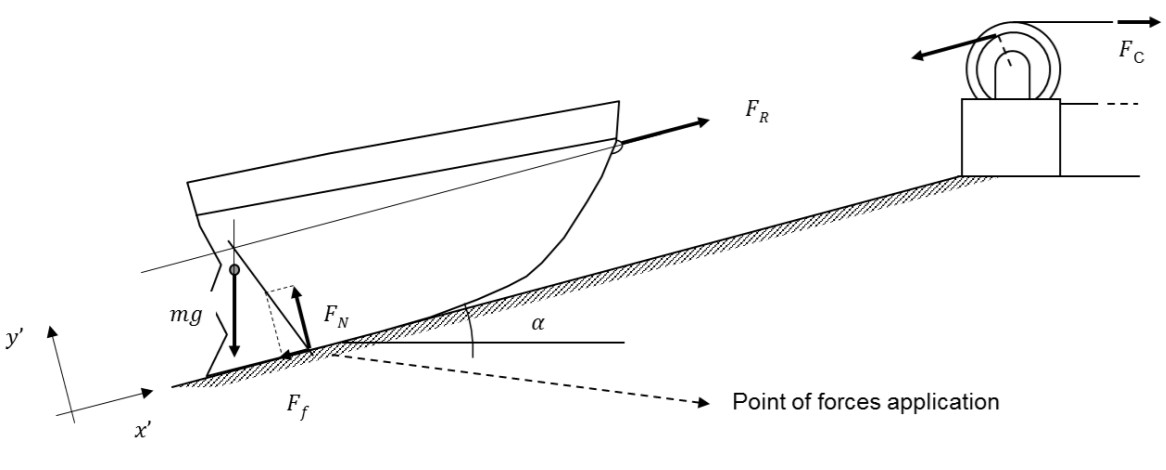
\includegraphics[width=0.8\linewidth]{boat-a}
		\caption{loads exchanged between the boat and the winch.} \label{ex:boat-a}
	\end{figure}
	With that said it's possible to continue the analysis by determining the reactional forces due to the bearings; using the free body diagram in figure \ref{ex:boat-fbd}, the linear system to solve is
	\[ \begin{cases}
		R_{Ay} + R_{By} = F_{Ry}\\
		R_{Az} + F_{Rz} = R_{Bz} + F_c\\
		R_{Bz} (a+b+c) = R_{Az} a + F_{Rz} (a+b) \\
		R_{Ay} a + R_{By} (a+b+c) = F_{Ry} (a+b)
	\end{cases} \] \noindent

	\begin{SCfigure}[1][bt]
		\centering 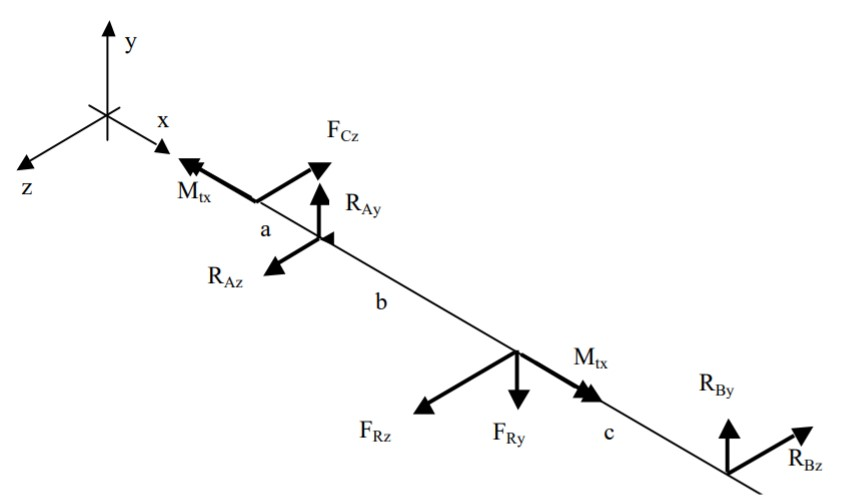
\includegraphics[width=10cm]{boat-b}
		\caption{free body diagram of the shaft} \label{ex:boat-fbd}
	\end{SCfigure}

	Knowing that $F_{Ry} = F_r \sin\alpha = 1\,389.45N$ and $F_{Rz} = F_r \cos\alpha = 2\,979.68 N$, such system can be solved depending on the geometrical parameters $a,b,c$:
	\[ R_{Ay} = \frac{c}{b+c} F_r \sin \alpha \qquad R_{Az} = \frac{(a+b+c)F_c - C F_r\cos\alpha}{b+c} \qquad R_{By} = \frac{b}{b+c} F_r\sin\alpha \qquad  R_{Bz} = \frac{a F_c + b F_r\cos\alpha}{b+c} \]
	Looking at the drawing of the problem, $a$ represent the length $L_1 - \frac s 2$, while both $b$ and $c$ depend on $L_x \in [0,L_5]$, in particular $b = \frac s 2 + L_2 + L_4 + L_x$ and $c = \frac s 2 + L_3-L_4-L_x$; in the two extremal situations we have
	\begin{center}
	\begin{tabular}{ M{1.5cm} | M{1cm} M{1cm} M{1cm} | M{1.5cm} M{1.5cm} M{1.5cm} M{1.5cm} }
		$L_x [mm]$ & $a [mm]$ & $b [mm]$ & $c [mm]$ & $R_{Ay} [N]$ & $R_{Az}[N]$ & $R_{By}[N]$ & $R_{Bz}[N]$ \\ \hline
		0 & \multirow{2}{*}{190} & 266 & 314 & 752.2 & 1005.7 & 637.2 & 2012.7 \\
		250 & & 516 & 64 & 153.3 & 2290.0 & 1236.1 & 3297.1		
	\end{tabular}
	\end{center}
	
	We can so proceed with the analysis of the internal action along the shaft; with the axis direction as shown in the free body diagram, it's possible to compute the shear components $V$ in the 3 main sections of the structure as described by the axis coordinate $\zeta$:
	\[ V_y = \begin{cases}
		0 & 0 < \zeta < a \\ R_{Ay} & a < \zeta < a+b \\
		-R_{By} & a+b < \zeta < a + b+ c
	\end{cases} \hspace{2cm} V_z = \begin{cases}
		-F_c & 0 < \zeta < a \\ R_{Az}+F_c & a < \zeta < a+b \\
		 R_{Bz}& a+b < \zeta < a + b+ c
	\end{cases}  \]
	and torsional moment
	\[ M_x = \begin{cases}
		F_c r_c & 0 < \zeta < a+b \\ 0 & a+b < \zeta < a+b+c
	\end{cases} \]
	More complex are the expressions for the bending moment that can be found by integration of the shear with the addition of boundary conditions, resulting in
	\[ M_z = \begin{cases}
		0 & 0 < \zeta < a \\ 
		R_{Ay} (\zeta-a) & a < \zeta < a+b \\
		R_{Ay} (\zeta-a) - F_{Ry} (\zeta-a-b) \qquad & a+b < \zeta < a + b+ c
	\end{cases} \] and \[ M_y = \begin{cases}
		-F_c \zeta & 0 < \zeta < a \\ -F_c\zeta + R_{Az}(\zeta-a) & a < \zeta < a+b \\
		-F_c\zeta + R_{Az}(\zeta-a) + F_{Rz}(\zeta-a-b) \qquad & a+b < \zeta < a + b+ c
	\end{cases}  \]
	
	\begin{figure}[bht]
		\centering
		\begin{subfigure}{0.48\linewidth}
			\centering 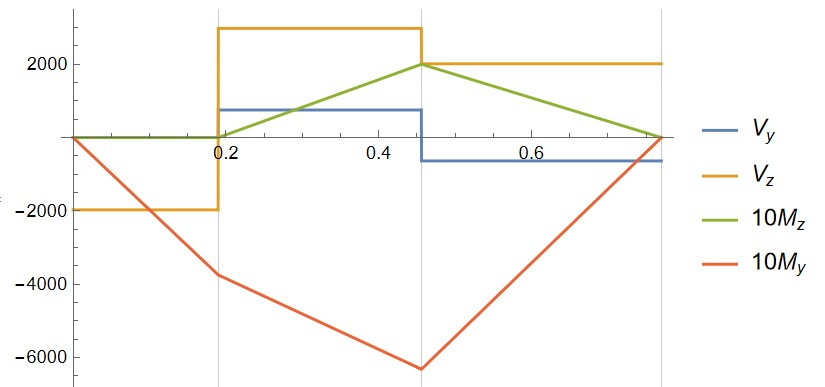
\includegraphics[width=\linewidth]{boat-intact-a} \caption{}
		\end{subfigure}
		\begin{subfigure}{0.48\linewidth}
			\centering 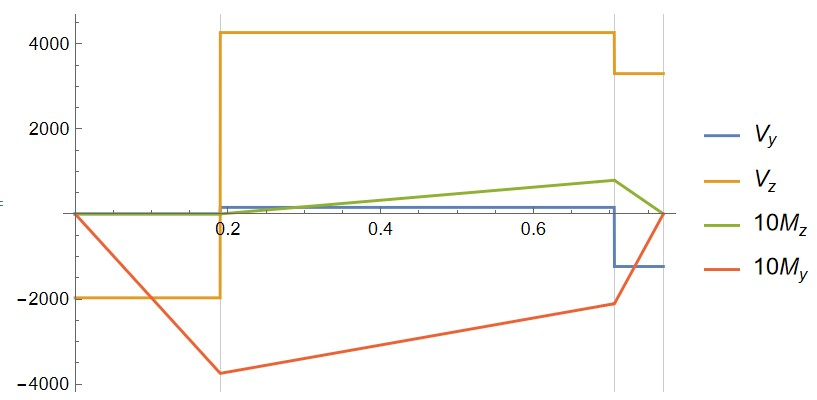
\includegraphics[width=\linewidth]{boat-intact-b} \caption{}
		\end{subfigure}
		\caption{internal action diagrams when $L_x=0$ (a) and $L_x = L_5 = 250mm$ (b).} \label{ex:boat:internal}
	\end{figure}
	By looking at the internal action diagram (figure \ref{ex:boat:internal}) and considering the shaft geometry, it can be notices that the most critical section can be regarded as the left side of the drum (point $E$ in figure \ref{ex:boat}); computing the internal action value for such point we have	
	\begin{center}
		\begin{tabular}{ M{1.5cm} | M{2cm} M{2cm} M{2cm} M{2cm}  M{2cm}  }
			$L_x [mm]$ & $V_y [N]$ & $V_z [N]$ & $M_x [N\cdot m]$ & $M_z [N\cdot m]$ & $M_y[N\cdot m]$ \\ \hline
			0 & 752 & 967 & \multirow{2}{*}{246.58} & 188.05 & -616.53    \\
			250 & 153 & -317 &  & 38.33 & -295.45
		\end{tabular}
	\end{center}
	From this table we can see that the most critical condition for point $E$ is for $L_x = 0$ (where bending has higher values) and so this case will be use in the prosecution of the exercise. Considering that the section has the property
	\[ A = \frac \pi 4 D_3^2 = 1963.5mm^2 \qquad I = \frac \pi {64} D_3^4 = 306\,796 mm^4 \qquad J_p = \frac \pi {32} D_3^4 = 613\,592 mm^4	 \]
	Due to the polar symmetry of the circular cross section it's possible to combine bending and shearing force components into vectors of amplitude
	\[ M_b = \sqrt{M_y^2+M_z^2} = 644.57 N \cdot m \hspace{2cm} V = \sqrt{V_y^2 + V_z^2} = 1\,225 N  \]
	Considering that the circular section has a shear factor $\chi = 4/3$, the maximum nominal stresses related to bending $\sigma$, the shear $\tau_s$ and torque $\tau_t$ are
	\[ \sigma = \frac{M_b}I \frac{D_3}2 = 52.5MPa \qquad \tau_s = \chi \frac V A = 0.83 MPa \qquad \tau_t = \frac{M_x}{J_p} \frac{D_3}{2} = 10MPa \]
	
	Having $\tau_s < 0.1 \sigma$ the stress component due to shear can be neglected for the fatigue (but if such expression wouldn't have been verified we should have summed two sinusoidal oscillating function $\sigma,\tau_s$ out of phase by $90^\circ$). During rotation $\tau_t$ remain constant throughout all the section while $\sigma$ varies following a (co)sinusoidal wave.\\
	To continue the analysis having $D/d = D_2 /D_3 = 1.2$ and $r/d = r/D_3 = 0.04$, from figure \ref{fig:stressconcentrationfactors} we retrieve the stress concentration factor $K_t = 2.08$ while with figure \ref{fig:notchsens} the notch sensitivity factor is $q = 0.82$, hence the notch fatigue factor is
	\[ K_f = 1 + q(K_t-1) = 1.89 \]
	This determines the effective amplitude component as
	\[ \sigma_{a,eff} = K_f \sigma = 99.2MPa \]
	The torsional stress is instead constant (static loading), therefore we only need to check that $\tau_{eff} = K_t \tau \leq = 16.7MPa \frac{\sys}{\sqrt 3}$ that's a verified inequality. If it wouldn't happen so a more complicated elastic-plastic analysis must have been required.
	
	To analyse the multiaxial loading we can use the Gough-Pollard criterion stating that the equivalent pure amplitude component can be regarded as
	\[ \sigma_{a,eq} = \sqrt{ \sigma_{a,eff}^2 + H^2 \tau_{eff}^2 } = \sqrt{\sigma_{a,eff}^2 + \left( \frac{C_s C_d C_l \sigma_{lim}}{\sys/\sqrt 3} \right)^2 \tau_t^2  } \leq \frac{C_sC_dC_l}{\phi} \sigma_{lim} \]
	
	In this case having a bending/torsion load then the related coefficient is $C_l = 1$; having a ground finished surface material then the associated coefficient (with parameters retrieved from table \ref{tab:surfacefinish}) becomes
	\[ C_s = a \suts^b = 1.58 \big(700\big)^{-0.085} = 0.9 \]
	Lastly having a circular section of diameter $d=50mm$, then the coefficient (using equation \ref{eq:dimensioncoefficient}) is $C_d = 1.189 d^{-0.097} = 0.82$. Having a $\sigma_{lim} = 360MPa$ and a yield $\sys = 450MPa$ then
	\[ \sall = \frac{C_sC_dC_l}{\phi} \sigma{lim} = \frac{267.5}{\phi} MPa \hspace{2cm} H = \frac{C_sC_dC_l \sigma_{lim}}{\sys/\sqrt 3} = 1.023 \]
	Inverting the equality $\sigma_{a,eq} = \frac \sys \phi$ it's possible to compute the safety factor against infinite lifetime fatigue as
	\[ \phi = \frac {C_sC_dC_l\sigma_{lim}}{\sqrt{ \sigma_{a,eff}^2 + H^2 \tau_{eff}^2 }} = 2.64\]
	
	
	
	
	
	
	
	
	
	
	
	